\chapter{Introduction}
\label{ch:Introduction}

\paragraph{ }The aim of technology review is to understand the working of all the tools and technologies relevant for this project.

To achieve this, tasks were assigned to each of the team to review few set of tools as below. 

\begin{figure} [h]
\centering
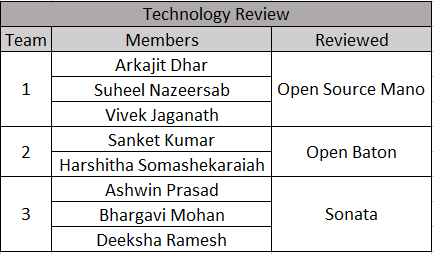
\includegraphics[width=.5\linewidth]{figures/teams}
\end{figure}

MANO frameworks such as Open Source MANO, Sonata and Open Baton have been reviewed in this phase. Different virtual infrastructure managers are tried and worked upon , like Kubernetes and Open Stack.\\*

The MANO frameworks are up and running in virtual machines and the connections are established between MANO and VIM's.\\*

The detailed explanation on installation and steps are given below in the document.



